\documentclass[serif, aspectratio=169]{beamer}
\usepackage[T1]{fontenc} 
\usepackage[utf8]{inputenc}
\usepackage[portuguese]{babel}
\usepackage{fourier}
\usepackage{hyperref}
\usepackage{bookmark}
\usepackage{latexsym,amsmath,xcolor,multicol,booktabs,calligra}
\usepackage{graphicx,pstricks,listings,stackengine}
\usepackage{lipsum}
\usepackage[linesnumbered,ruled,vlined]{algorithm2e}
\usepackage{UFCStyle}

% Definições visuais
\definecolor{hkustyellow}{RGB}{167, 131, 55}
\definecolor{hkustblue}{RGB}{0, 56, 116}
\definecolor{hkustred}{RGB}{209, 51, 59}

\lstset{
    basicstyle=\ttfamily\small,
    keywordstyle=\bfseries\color{deepblue},
    emphstyle=\ttfamily\color{deepred},
    stringstyle=\color{deepgreen},
    numbers=left,
    numberstyle=\small\color{halfgray},
    rulesepcolor=\color{red!20!green!20!blue!20},
    frame=shadowbox,
}

% Informações da apresentação
\title{Trabalho Final - Probabilidade e Estatística (2025.2)}
\subtitle{Equipe 02}
\author{
Ismael S. Silva, Paulo R. S. Menezes, Ana N. M. de Araujo\and
Kaique D. Sousa, Wanessa R. Santos, Eros R. Simette\and
Thiago C. S. Oliveira, Pedro H. Q. da Silva\and
Marcos G. P. Galdino, Luiz M. R. de Souza, Adrian E. O. Azevedo
}
\institute{Universidade Federal do Ceará}
\date{\small \today}

% Comandos customizados
\def\cmd#1{\texttt{\color{red}\footnotesize $\backslash$#1}}
\def\env#1{\texttt{\color{blue}\footnotesize #1}}

\lstdefinelanguage{Portugol}{
    morekeywords={
        para, se, entao, fim, enquanto, funcao, retorna, inteiro, vetor, inicio,
        verdadeiro, falso, cada, faca, repita, ate, caso, senao, escreva, leia
    },
    sensitive=true,
    morecomment=[l]{//},
    morestring=[b]",
}

% Definição do estilo para o Portugol
\lstdefinelanguage{Portugol}{
    morekeywords={
        para, se, entao, fim, enquanto, funcao, retorna, inteiro, vetor, inicio,
        verdadeiro, falso, cada, faca, repita, ate, caso, senao, escreva, leia
    },
    sensitive=true,
    morecomment=[l]{//},
    morestring=[b]",
}

\lstdefinestyle{portugolStyle}{
    language=Portugol,
    basicstyle=\ttfamily\small,
    keywordstyle=\color{blue}\bfseries,
    commentstyle=\color{gray}\itshape,
    stringstyle=\color{orange},
    numbers=none,
    numberstyle=\tiny\color{gray},
    stepnumber=1,
    numbersep=8pt,
    backgroundcolor=\color{white},
    showspaces=false,
    showstringspaces=false,
    showtabs=false,
    frame=single,
    breaklines=true,
    tabsize=4,
    captionpos=b
}

% --- Início do documento ---
\begin{document}

% Slide de título
\begin{frame}
    \titlepage
    \vspace*{-0.6cm}
    \begin{figure}[htpb]
        \begin{center}
            
\includegraphics[keepaspectratio, scale=0.06]{figures/UFC.png}
        \end{center}
    \end{figure}
\end{frame}

% Sumário
\begin{frame}    
\tableofcontents[sectionstyle=show,
subsectionstyle=show/shaded/hide,
subsubsectionstyle=show/shaded/hide]
\end{frame}

% Seções modulares
\section{Introdução}
\section{Resolução Questão 2}

\section{Questão 4}

% -------------------------------
\begin{frame}{Descrição da Questão}
Considere que $X_1, X_2, \ldots, X_n$ são variáveis aleatórias independentes e identicamente distribuídas (i.i.d.) com distribuição uniforme contínua no intervalo $[0,6]$. Define-se a média amostral como:

\[
\bar{X} = \frac{1}{n} \sum_{i=1}^{n} X_i
\]

O objetivo é analisar o comportamento da média amostral com base em simulações e aplicar conceitos estatísticos, como o Teorema Central do Limite e Intervalos de Confiança.
\end{frame}

% -------------------------------
\begin{frame}[fragile]{Letra a) Geração das Amostras}
Geramos 1200 amostras de tamanho $n = 800$ da distribuição $U(0,6)$ utilizando a função \texttt{grand} do Scilab.

\vspace{0.3em}
\lstinputlisting[
    language=Scilab,
    basicstyle=\ttfamily\scriptsize,
    caption={questao04\_amostras\_ic.sci}
]{../q04/questao04_amostras_ic.sci}

\vspace{0.3em}
Como $U(0,6)$ tem média $\mu = 3$ e variância $\sigma^2 = 3$, o Teorema Central do Limite garante que $\bar{X}$ é aproximadamente normal para grandes $n$.
\end{frame}

% -------------------------------
\begin{frame}[fragile]{Letra b) Intervalos de Confiança}
Utilizando o Teorema Central do Limite e o desvio padrão amostral $s$, construímos intervalos de confiança com níveis de 90\%, 95\% e 99\%:

\[
IC = \left( \bar{X} \pm z_\alpha \cdot \frac{s}{\sqrt{n}} \right)
\]

\vspace{0.3em}
\lstinputlisting[
    language=Scilab,
    basicstyle=\ttfamily\scriptsize,
    caption={questao04\_calculo\_ic.sci}
]{../q04/questao04_calculo_ic.sci}

\vspace{0.3em}
Com valores:
\begin{itemize}
  \item $z_{0.90} = 1.645$
  \item $z_{0.95} = 1.960$
  \item $z_{0.99} = 2.576$
\end{itemize}
\end{frame}

% -------------------------------
\begin{frame}[fragile]{Letra c) Proporção de Intervalos que Contêm $\mu = 3$}
Verificamos a proporção de intervalos que efetivamente contêm o valor da média verdadeira.

\vspace{0.3em}
\lstinputlisting[
    language=Scilab,
    basicstyle=\ttfamily\scriptsize,
    caption={questao04\_percentual\_contem\_media.sci}
]{../q04/questao04_percentual_contem_media.sci}
\end{frame}

% -------------------------------
\begin{frame}{Conclusão}
\begin{itemize}
  \item A média das amostras geradas de $U(0,6)$ segue, aproximadamente, uma distribuição normal conforme previsto pelo Teorema Central do Limite.
  \item Os intervalos de confiança calculados mostram boa consistência com os níveis de confiança estipulados.
  \item Quanto maior o nível de confiança, mais largo o intervalo e maior a probabilidade de conter a média populacional.
\end{itemize}
\end{frame}

\section{Resolução Questão 12} 

\section{Resolução Questão 17}

\begin{frame}{Questão 17}
Considere um programa de TV em que um participante deve escolher uma de três portas. Atrás de uma das portas existe um carro, enquanto nada existe atrás das outras duas.

\vspace{0.3cm}
A produção coloca o prêmio de forma aleatória atrás de uma das portas. Após a escolha de uma porta, o apresentador abre uma das outras portas que não contém o prêmio, e pergunta ao participante se ele deseja trocar sua escolha.
\end{frame}

% Slide 2: Portas
\begin{frame}{Qual porta escolher?}
\centering
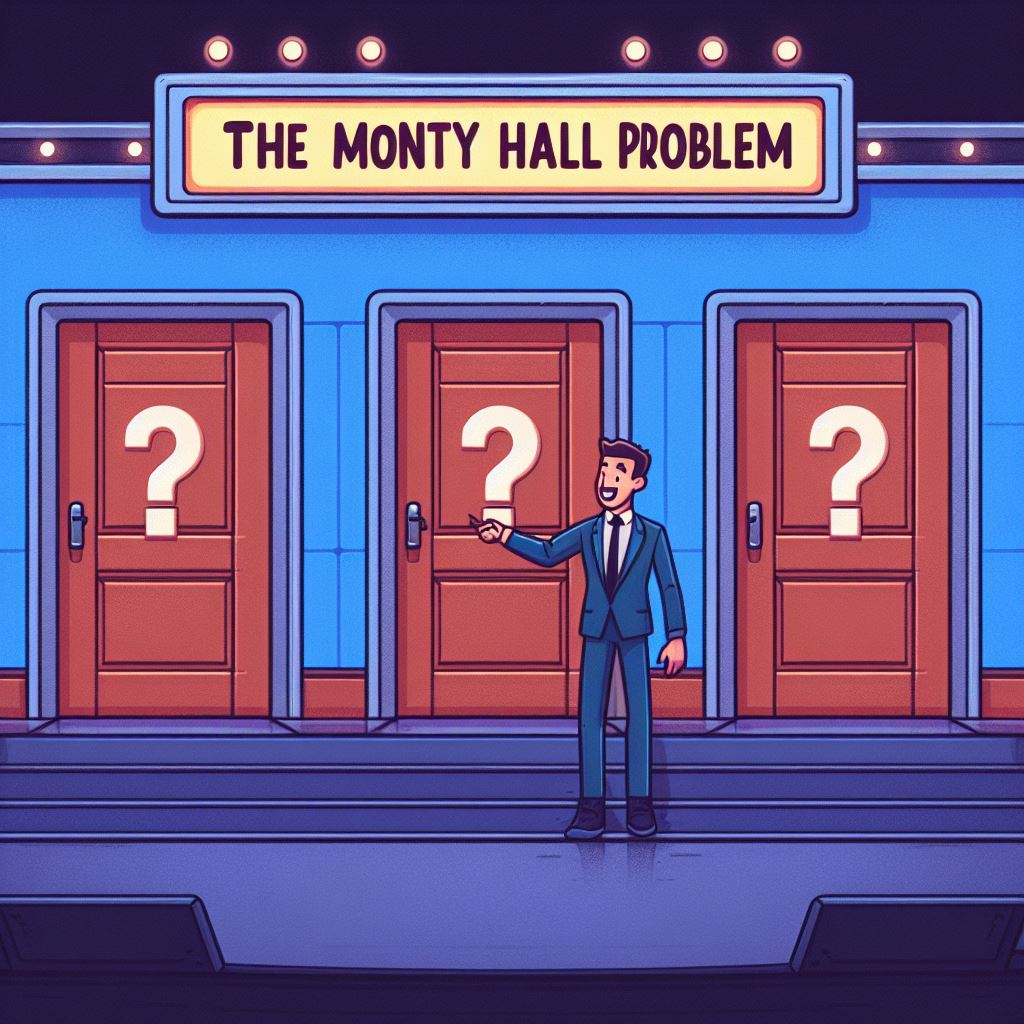
\includegraphics[width=0.45\textwidth]{figures/MontyHall.jpeg}
\end{frame}

% Slide 3: Código
\begin{frame}[fragile]{Simulação}
 \begin{figure}
    \centering
    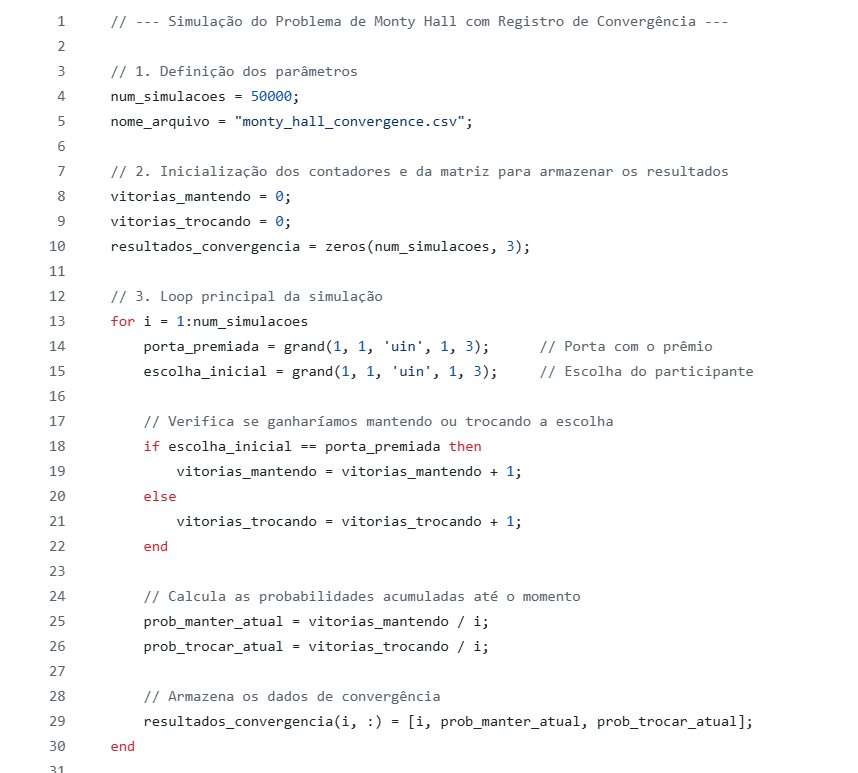
\includegraphics[width=0.9\linewidth]{figures/Captura de tela 2025-07-18 154707.png}
 \end{figure}
\end{frame}

\begin{frame}[fragile]{Simulação}
 \begin{figure}
    \centering
    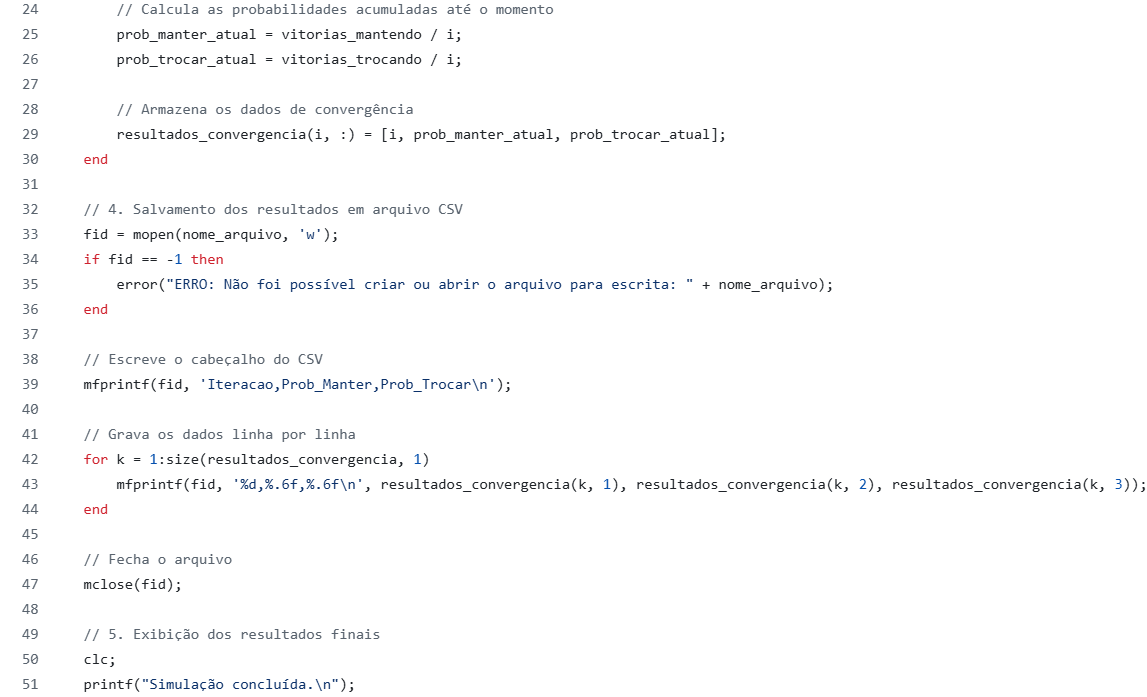
\includegraphics[width=0.9\linewidth]{figures/parte ok 2.png}
 \end{figure}
\end{frame}

\begin{frame}[fragile]{Simulação}
 \begin{figure}
    \centering
    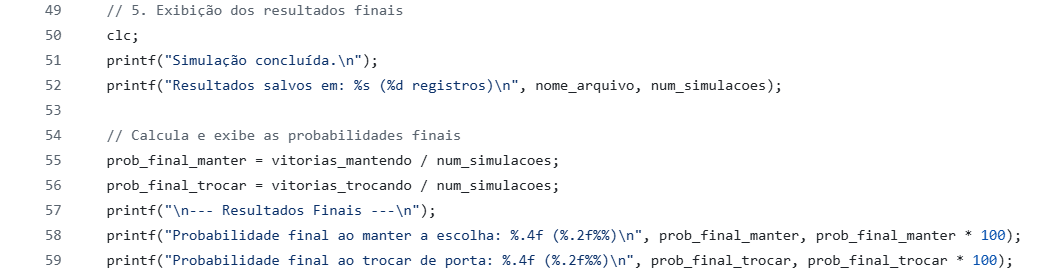
\includegraphics[width=0.9\linewidth]{figures/Captura de tela 2025-07-18 160019.png}
 \end{figure}
\end{frame}

\begin{frame}[fragile]{Convergência}
 \begin{figure}
    \centering
    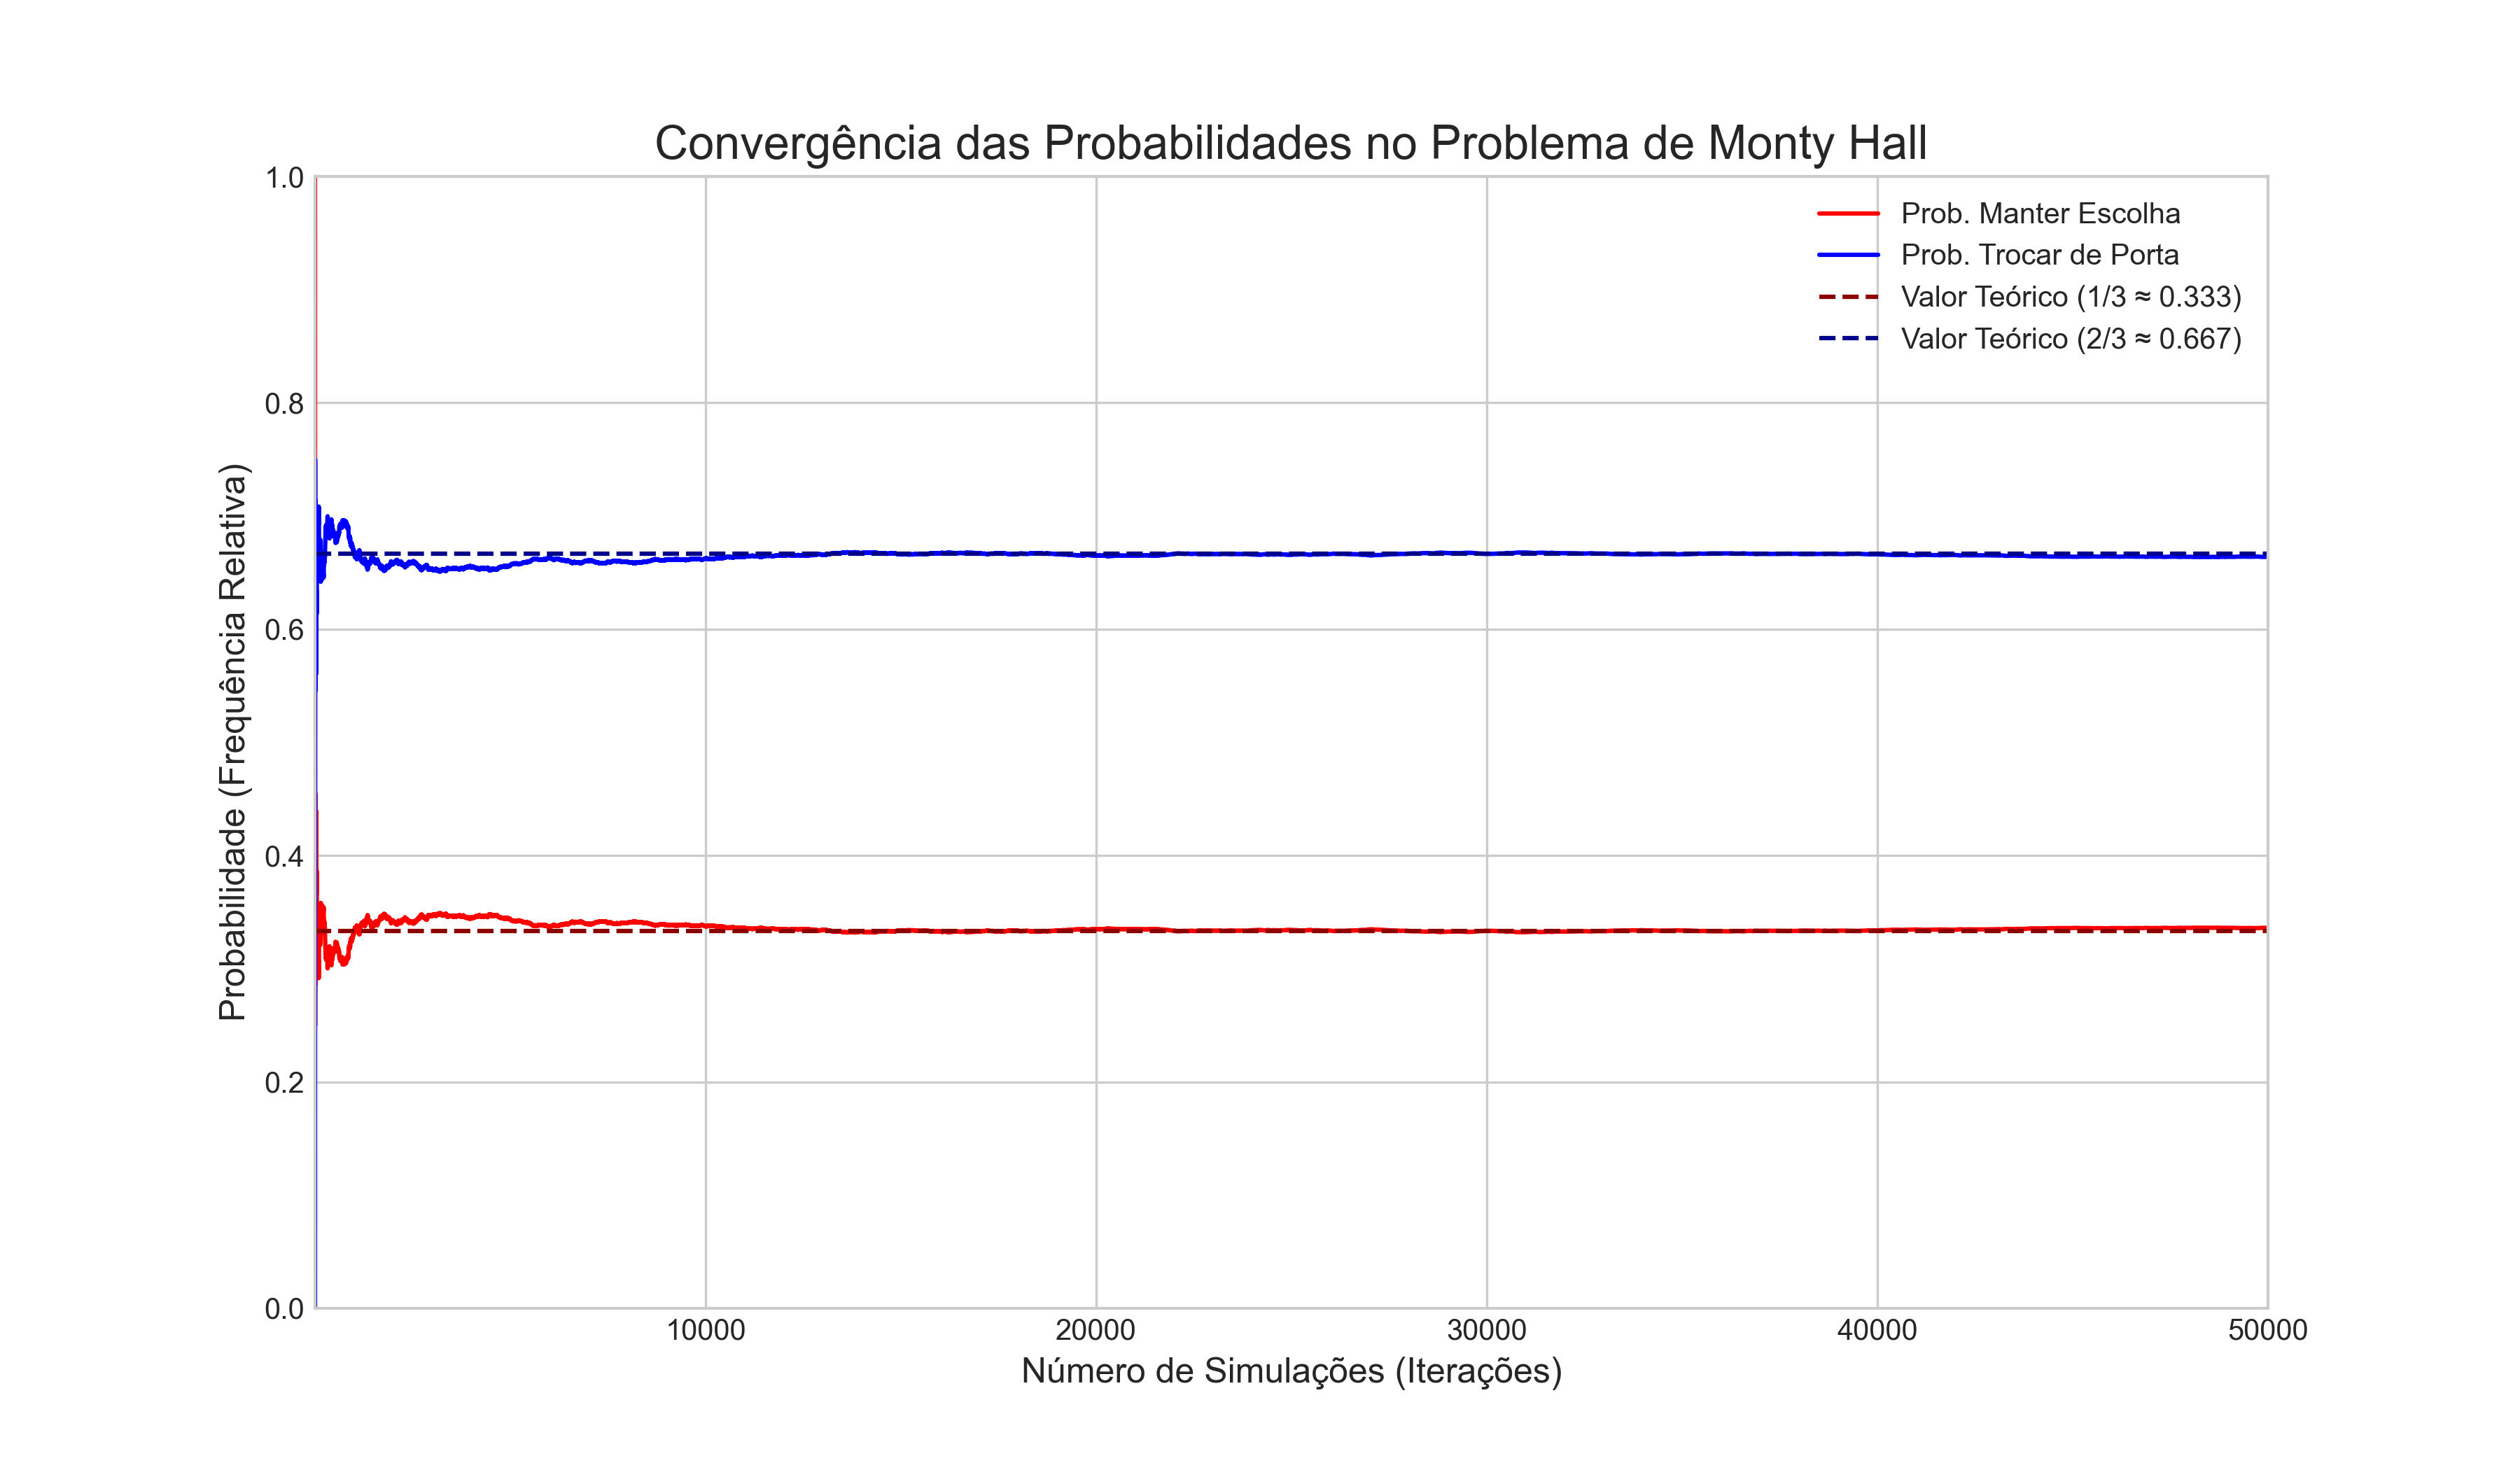
\includegraphics[width=0.9\linewidth]{figures/convergencia_monty_hall.png}
 \end{figure}
\end{frame}

% Slide 5: Código - Trocando
\begin{frame}[fragile]{Sempre trocando de porta}
A resposta intuitiva ao problema é a que quando o apresentador revelou uma das portas não premiadas, o participante passaria a ter um novo dilema com duas portas e um prêmio. Portanto, a chance do prêmio estar em uma das portas seria 1/2. 
 
A resposta contra-intuitiva e certa é que é mais vantajoso trocar, pois a
chance de ganhar trocando é o dobro da chance de ganhar sem trocar
\begin{figure}
    \centering
    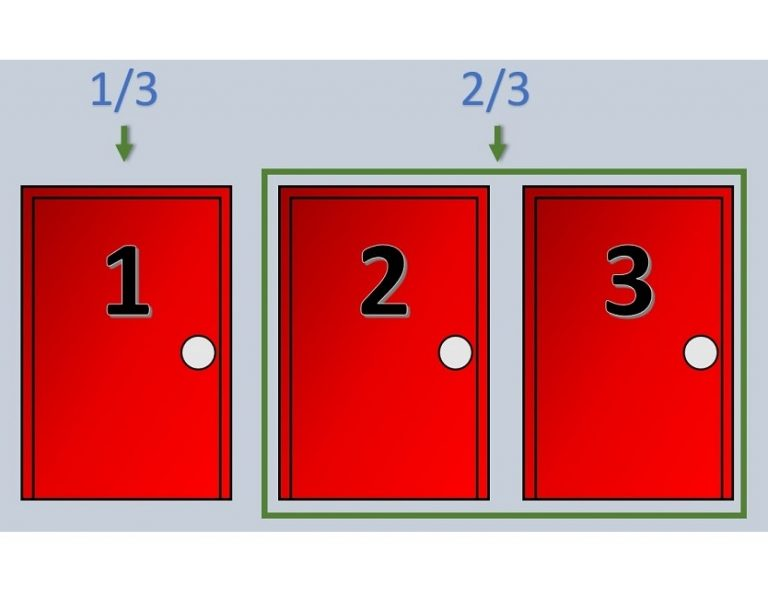
\includegraphics[width=0.45\linewidth]{figures/porc portas.jpg}
    \label{fig:enter-label}
 \end{figure}
\end{frame}
% Slide 6: Resultado
\begin{frame}{Solução}
\textbf{Resposta correta: é melhor trocar de porta!}

\vspace{0.3cm}
\begin{itemize}
  \item Probabilidade de ganhar sem trocar: \textbf{1/3}
  \item Probabilidade de ganhar trocando: \textbf{2/3}
\end{itemize}

\vspace{0.4cm}
\centering
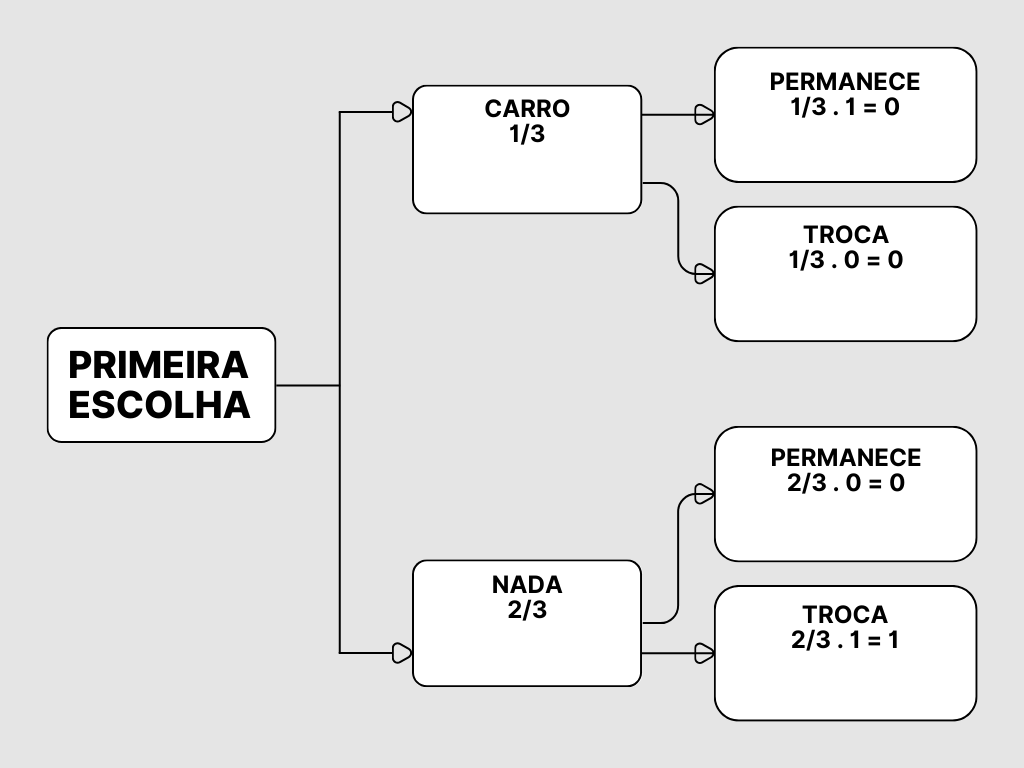
\includegraphics[width=0.4\textwidth]{figures/Grey and White Minimalist Simple Concept Map.png} 
\end{frame}
\section{Conclusão}

\section{Referências Bibliográficas}

\begin{frame}[allowframebreaks]
    \frametitle{Referências Bibliográficas}

    \begin{itemize}
        \item MONTGOMERY, D. C.; RUNGER, G. C. *Estatística Aplicada e Probabilidade para Engenheiros*. 6ª ed. LTC, 2016.

        \item ROSS, S. M. *Probabilidade e Estatística para Engenharia e Ciências*. 9ª ed. Elsevier, 2018.

        \item WASSERMAN, L. *All of Statistics: A Concise Course in Statistical Inference*. Springer, 2004.

        \item PAPOULIS, A.; PILLAI, S. U. *Probability, Random Variables and Stochastic Processes*. McGraw-Hill, 2002.

        \item GRIMMETT, G.; STIRZAKER, D. *Probability and Random Processes*. Oxford University Press, 3ª ed., 2001.
    \end{itemize}

\end{frame}

% Slide final
\begin{frame}
\begin{center}
{\Huge Obrigado pela atenção!}
\vspace{1cm}

\end{center}
\end{frame}

\end{document}
